% !TEX root = main.tex

\chapter{試料構造と測定方法}
%\label{chap:simulation}

\section{はじめに}

\section{試料作製}
\subsection{試料構造}
\subsection{ブロードコンタクトレーザー}
\subsection{リッジ導波路型レーザー}
\subsection{マウント(ダイボンディング??)}
\section{測定方法}
本研究ではエピウエハの品質評価のための測定と利得スイッチング動作を起こしデバイスの高速特性を評価するための測定を行った。
\subsection{定常電流注入による測定実験}
まずエピウエハの品質を調べるために定常電流を注入する実験を行った。発振閾値電流や発振閾値電流密度などの基本的な物性パラメータを見積もることができる。
実験系を図\ref{fig:IL}に示す。パルスジェネレータから数usパルスを数ms周期で発生させ、試料に注入する。ここでマイクロ秒程度のパルスは試料の中での発光過程やその他の物理現象の時間オーダーに対して十分長く、定常電流とみなすことができる。DC電流では熱の影響が大きくなってしまい試料が壊れてしまう恐れがあるため。Duty比(パルス幅と繰り返し周期の比)を1:1000程度に設定して実験を行った。試料からの発光強度を光パワーメータで測定した。また、回路に試料と並列に抵抗(22.4オーム)を入れ、そこにかかる電圧をモニタすることで流れる電流量および、試料にかかる電圧を測定した。試料にかかる電圧は回路全体にかかる電圧と抵抗にかかる電圧の差を取ることにより算出した。
\begin{figure}[htbp]
	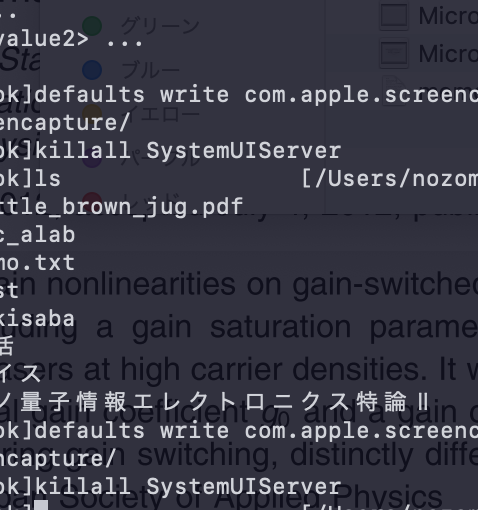
\includegraphics[width=15cm]{test_fig.png}
	\caption{test}
	\label{fig:IL}
\end{figure}
\subsection{電流注入利得スイッチング実験}
ナノ秒程度の短いパルス電圧を印可し、測定を行う実験系の模式図を図\ref{fig:GS_setup}に示す。パルスジェネレータから同軸ケーブルを介して試料へ電気パルスが印加される。試料からの発光は対物レンズでコリメートされ、非球面レンズで光ファイバーに集光される。その後フォトダイオードで検出しその電圧を高速オシロスコープでモニタした。
\begin{figure}[htbp]
	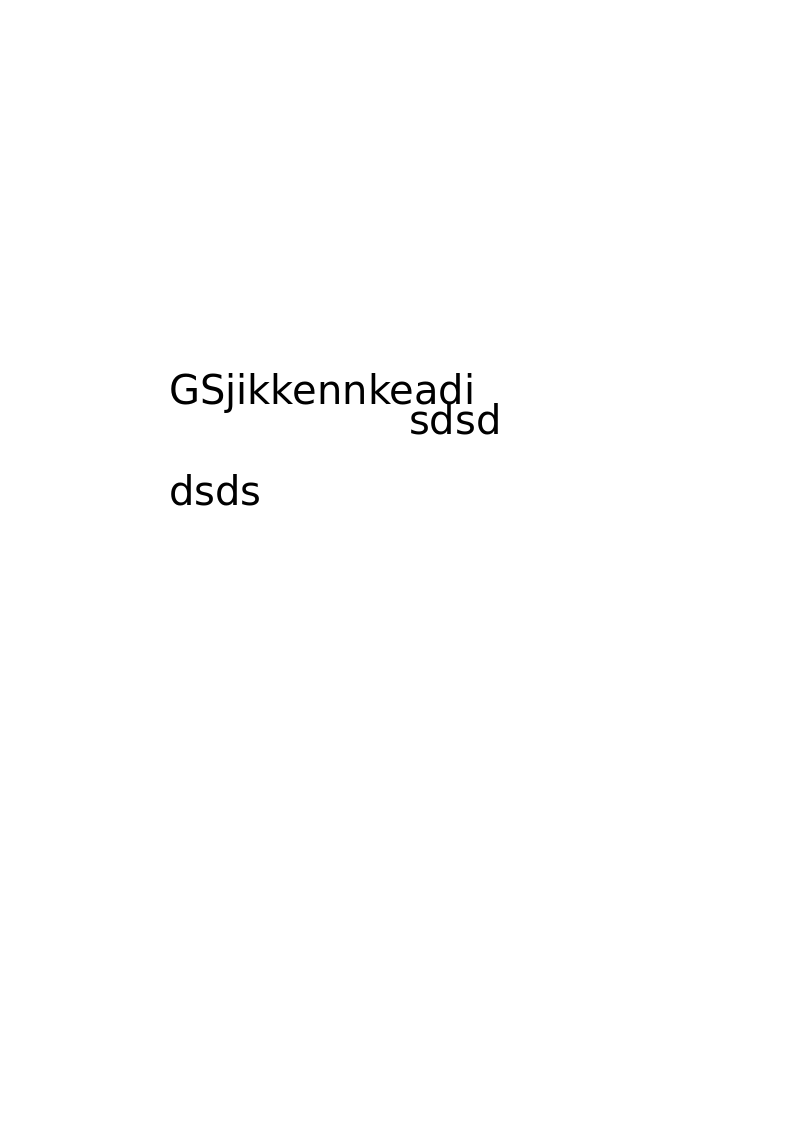
\includegraphics[width=15cm]{../a/GS_setup.png}
	\caption{GS実験}
	\label{fig:GS_setup}
\end{figure}


